\documentclass[14pt]{beamer}
\usepackage{./Estilos/BeamerUVM}
\usepackage{./Estilos/ColoresLatex}
%Sección para el tema de beamer, con el theme, usercolortheme y sección de footers
\usetheme{Berlin}
\usecolortheme{beaver}
%\useoutertheme{default}
\setbeamercovered{invisible}
% or whatever (possibly just delete it)
\setbeamertemplate{section in toc}[sections numbered]
\setbeamertemplate{subsection in toc}[subsections numbered]
\setbeamertemplate{subsection in toc}{\leavevmode\leftskip=3.2em\rlap{\hskip-2em\inserttocsectionnumber.\inserttocsubsectionnumber}\inserttocsubsection\par}
% \setbeamercolor{section in toc}{fg=blue}
% \setbeamercolor{subsection in toc}{fg=blue}
% \setbeamercolor{frametitle}{fg=blue}
% \setbeamertemplate{caption}[numbered]

\setbeamertemplate{footline}
\beamertemplatenavigationsymbolsempty
\setbeamertemplate{headline}{}


\makeatletter
% \setbeamercolor{section in foot}{bg=gray!30, fg=black!90!orange}
% \setbeamercolor{subsection in foot}{bg=blue!30!yellow, fg=red}
% \setbeamercolor{date in foot}{bg=black, fg=white}
\setbeamertemplate{footline}
{
  \leavevmode%
  \hbox{%
  \begin{beamercolorbox}[wd=.333333\paperwidth,ht=2.25ex,dp=1ex,center]{section in foot}%
    \usebeamerfont{section in foot} \insertsection
  \end{beamercolorbox}%
  \begin{beamercolorbox}[wd=.333333\paperwidth,ht=2.25ex,dp=1ex,center]{subsection in foot}%
    \usebeamerfont{subsection in foot}  \insertsubsection
  \end{beamercolorbox}%
  \begin{beamercolorbox}[wd=.333333\paperwidth,ht=2.25ex,dp=1ex,right]{date in head/foot}%
    \usebeamerfont{date in head/foot} \insertshortdate{} \hspace*{2em}
    \insertframenumber{} / \inserttotalframenumber \hspace*{2ex} 
  \end{beamercolorbox}}%
  \vskip0pt%
}

% \usefonttheme{serif}
\usepackage[clock]{ifsym}
\DeclareSIUnit\erg{erg}
\DeclareSIUnit[number-unit-product = {\,}]\cal{cal}

\sisetup{per-mode=symbol}
\resetcounteronoverlays{saveenumi}

% Macro para agregar el logo de UVM en cada slide de la presentación

\addtobeamertemplate{frametitle}{}{%
\begin{tikzpicture}[remember picture,overlay]
\coordinate (logo) at ([xshift=-1.5cm,yshift=-0.8cm]current page.north east);
% \fill[devryblue] (logo) circle (.9cm);
% \clip (logo) circle (.75cm);
\node at (logo) {
\includegraphics[width=2.1cm]{Imagenes/logo_UVM.png}};
\end{tikzpicture}}


\title{\Large{Calor, Trabajo y Energía} \\ \normalsize{Física III}}
\date{}

\begin{document}
\maketitle

\section*{Contenido}
\frame[allowframebreaks]{\frametitle{Contenido} \tableofcontents[currentsection, hideallsubsections]}

\section{Trabajo en física}
\frame[allowframebreaks]{\tableofcontents[currentsection, hideothersubsections]}
\subsection{Definición}

\begin{frame}
\frametitle{El concepto de Energía}
El concepto de \textocolor{blue-violet}{energía} es fundamental en la física \pause y se refiere a la \textocolor{indigo(web)}{capacidad de un sistema para realizar trabajo}.
\end{frame}
% \begin{frame}
% \frametitle{Transformando la energía}
% La energía puede manifestarse de diferentes formas y puede ser \textocolor{red}{transformada} de una forma a otra.
% \end{frame}
% \begin{frame}
% \frametitle{Transformando la energía}
% La \textocolor{cobalt}{cantidad total de energía} en un sistema aislado \textocolor{cobalt}{se conserva}, \pause de acuerdo con el principio de conservación de la energía.
% \end{frame}
% \begin{frame}
% \frametitle{Ejemplo de transformación}
% En el motor de automóvil, \pause la energía química almacenada en el combustible se convierte parcialmente en la energía del movimiento del auto, \pause y parcialmente en energía térmica.
% \end{frame}
% \begin{frame}
% \frametitle{Ejemplo de transformación}    
% \begin{figure}
%     \centering
%     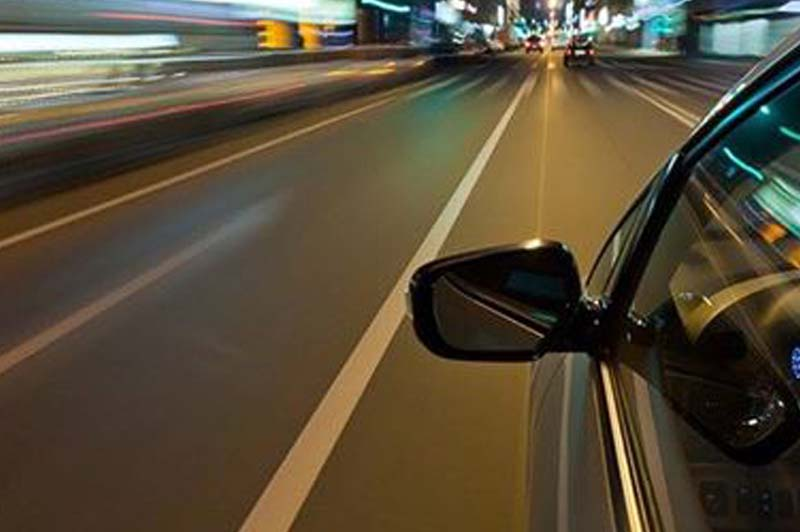
\includegraphics[scale=0.3]{Imagenes/Energia_01.jpg}
% \end{figure}
% \end{frame}
% \begin{frame}
% \frametitle{Ejemplo de transformación}    
% En un horno de microondas, la energía electromagnética obtenida de la CFE se convierte en energía térmica en el alimento caliente o cocido.
% \end{frame}
% \begin{frame}
% \frametitle{Ejemplo de transformación}
% \vspace*{-1cm} 
% \begin{figure}
%     \centering
%     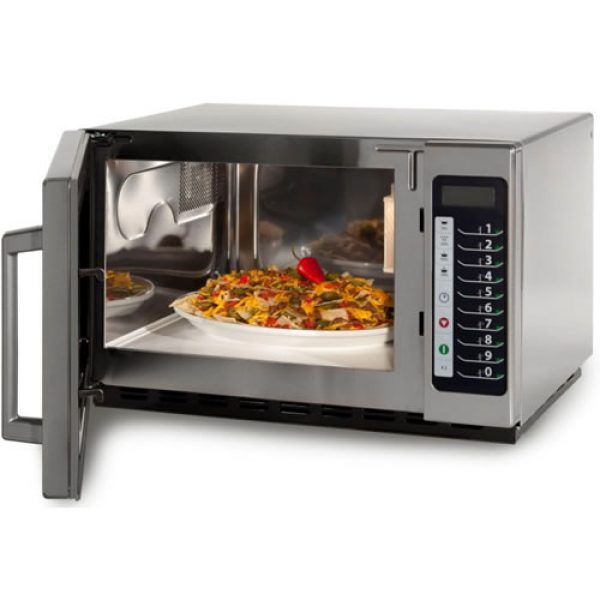
\includegraphics[scale=0.3]{Imagenes/Energia_02.jpg}
% \end{figure}
% \end{frame}

% \subsection{Conceptos clave}

% \begin{frame}
% \frametitle{El trabajo mecánico}
% El \textocolor{americanrose}{trabajo mecánico (T)} se refiere a la transferencia de energía de un objeto a otro debido a una fuerza aplicada a lo largo de una distancia.
% \end{frame}
% \begin{frame}
% \frametitle{Energía cinética}
% La \textocolor{ao(english)}{energía cinética $(E_{k})$} se refiere a la energía asociada al movimiento de un objeto.
% \pause
% \begin{align*}
% E_{k} = \dfrac{1}{2} m \, v^{2}
% \end{align*}
% \end{frame}
% \begin{frame}
% \frametitle{Energía cinética}
% \vspace*{-1cm}
% \begin{figure}
%     \centering
%     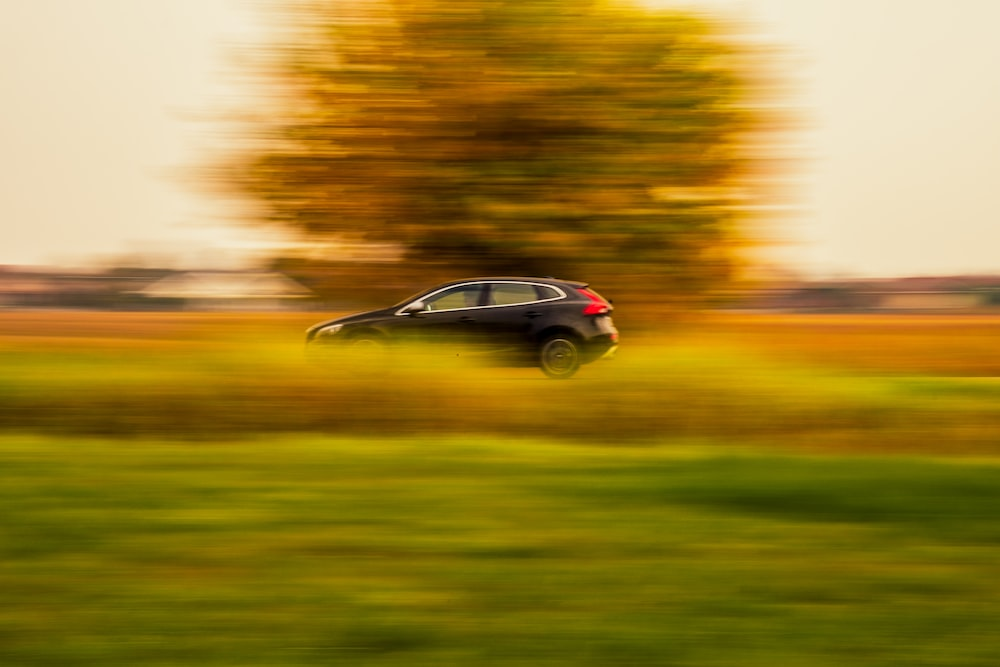
\includegraphics[scale=0.2]{Imagenes/Energia_cinetica_01.jpg}
% \end{figure}
% \end{frame}
% \begin{frame}
% \frametitle{Energía potencial}
% La \textocolor{blue(pigment)}{energía potencial $(E_{p})$} es la energía asociada con la posición o el estado de un objeto.
% \pause
% \begin{align*}
% E_{p} = m \, g \,  h
% \end{align*}
% \end{frame}
% \begin{frame}
% \frametitle{Energía potencial}
% \vspace*{-1cm}
% \begin{figure}
%     \centering
%     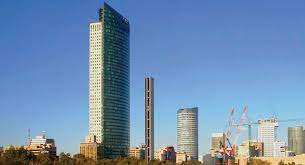
\includegraphics[scale=0.7]{Imagenes/Energia_potencial_01.jpg}
% \end{figure}
% \end{frame}
% \begin{frame}
% \frametitle{Energía mecánica}
% La \textocolor{bronze!10!black}{energía mecánica $(E_{T})$} es la suma de la \textocolor{ao(english)}{energía cinética} y la \textocolor{blue(pigment)}{energía potencial} de un objeto en un sistema. 
% \begin{align*}
% E_{t} = E_{k} + E_{p}
% \end{align*}
% \end{frame}
% \begin{frame}
% \frametitle{Energía térmica}
% La \textocolor{burntumber}{energía térmica} se refiere a la energía asociada con la temperatura de un objeto o un sistema.
% \begin{figure}
%     \centering
%     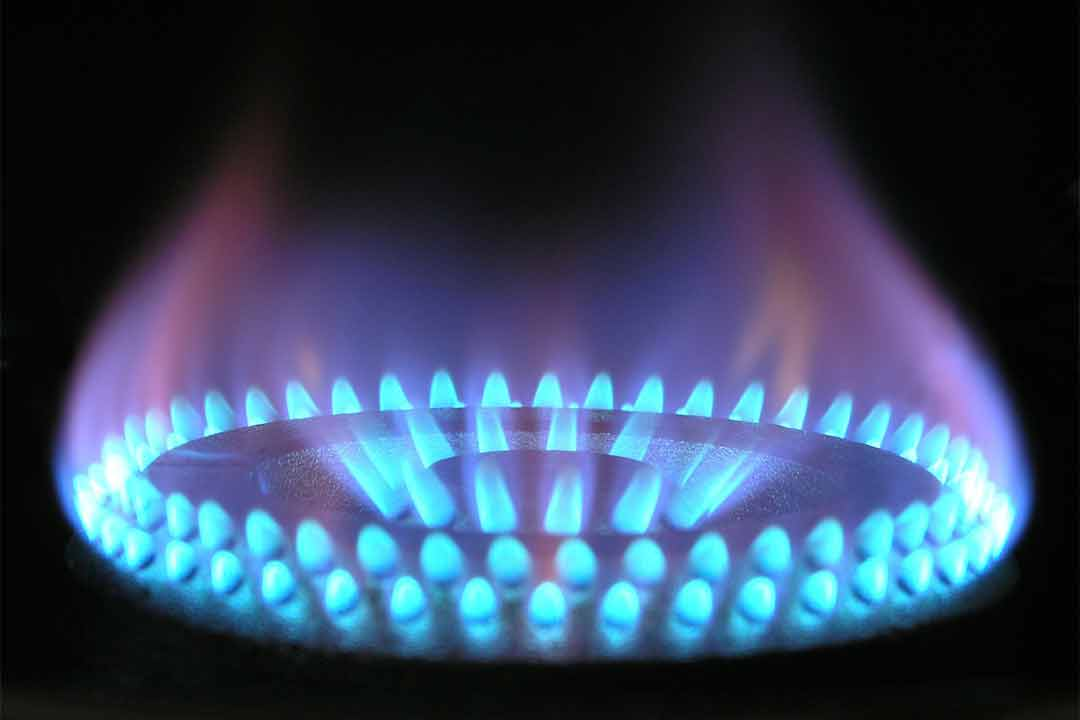
\includegraphics[scale=0.15]{Imagenes/Energia_termica_01.jpg}
% \end{figure}
% \end{frame}
% \begin{frame}
% \frametitle{Ley de conservación de la energía}
% La energía total de un sistema aislado se mantiene constante. 
% \end{frame}

\subsection{Trabajo mecánico}

\begin{frame}
\frametitle{Comprendiendo el trabajo}
Podemos pensar en el \textocolor{bole}{trabajo mecánico}, cuando vemos a una persona transportar un objeto pesado o cuando subimos las escaleras.
\\
\bigskip
\pause
Realizar un trabajo implica consumir energía.
\end{frame}
\begin{frame}
\frametitle{Comprendiendo el trabajo}
\begin{figure}
    \centering
    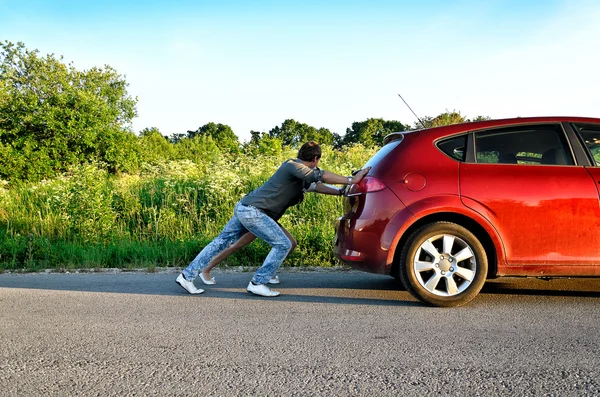
\includegraphics[scale=0.4]{Imagenes/Energia_03.png}
\end{figure}
\end{frame}
\begin{frame}
\frametitle{Factores en el trabajo}
En todos los casos en los que se realiza un trabajo, intervienen tres factores:
\pause
\setbeamercolor{item projected}{bg=darkred,fg=white}
\setbeamertemplate{enumerate items}{%
\usebeamercolor[bg]{item projected}%
\raisebox{1.5pt}{\colorbox{bg}{\color{fg}\footnotesize\insertenumlabel}}%
}
\begin{enumerate}[<+->]
\item La aplicación de una fuerza.
\item El desplazamiento.
\item Una componente a lo largo del desplazamiento.
\end{enumerate}
\end{frame}
\begin{frame}
\frametitle{Consideraciones para la definición}
Si se considera que la fuerza es constante y el movimiento es en línea recta y en la dirección de la fuerza.
\end{frame}
\begin{frame}
\frametitle{Definición del trabajo mecánico}
Entonces el \textocolor{blue}{trabajo mecánico} que realiza la fuerza aplicada sobre un objeto \pause se define como \textocolor{lava}{el producto de la fuerza por distancia que recorre el objeto}.
\end{frame}
\begin{frame}
\frametitle{Expresión para el trabajo}
\vspace*{-1cm}
La expresión es:
\begin{align*}
T = F \cdot d \hspace{0.5cm} \rightarrow \hspace{0.5cm} \left[ J \quad (\text{Joule}) \right]
\end{align*}
\pause
Donde:
\setbeamercolor{item projected}{bg=deepcarmine,fg=white}
\setbeamertemplate{enumerate items}{%
\usebeamercolor[bg]{item projected}%
\raisebox{1.5pt}{\colorbox{bg}{\color{fg}\footnotesize\insertenumlabel}}%
}
\begin{enumerate}[<+->]
\item $F$ es la fuerza (en Newtons)
\item $d$ es la distancia (en metros)
\item $T$ es el trabajo medido en Joules (Newton por metro)
\end{enumerate}
\end{frame}
\begin{frame}
\frametitle{Consideración de las unidades}
Haciendo una descripción completa de las unidades, se tiene que:
\begin{eqnarray*}
\begin{aligned}
\si{\joule} = \pause \si{\newton\meter} = \pause \si[per-mode=fraction]{\kilo\gram\meter\per\square\second} \cdot \si\meter = \pause \si[per-mode=fraction]{\kilo\gram\square\meter\per\square\second}
\end{aligned}
\end{eqnarray*}
\end{frame}
\begin{frame}
\frametitle{Triángulo del Trabajo}
\begin{figure}
    \centering
    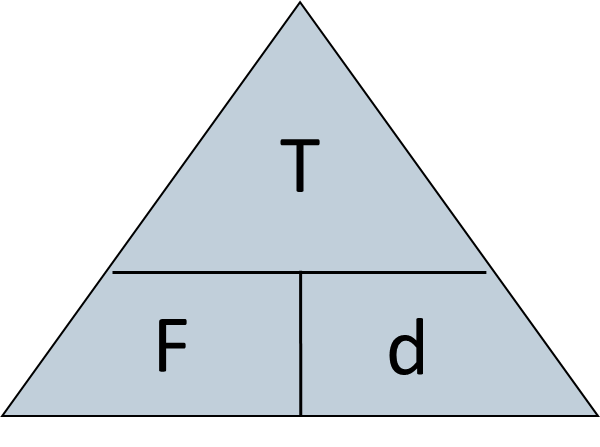
\includegraphics[scale=1]{Imagenes/Triangulo_Trabajo.png}
\end{figure}
\end{frame}
\begin{frame}
\frametitle{Enunciado del Ejercicio}
Un barco remolcador ejerce una fuerza constante de \SI{5000}{\newton} sobre un barco que se mueve con  velocidad constante a través del mar.
\\
\bigskip
\pause
¿Cuánto trabajo hace el remolcador sobre el barco en una distancia de \SI{3}{\kilo\meter}?
\end{frame}
\begin{frame}
\frametitle{Resolviendo el ejercicio}
\textocolor{red}{Datos:}
\pause
\begin{align*}
F &= \SI{5000}{\newton} \\[0.5em]
d &= \SI{3}{\kilo\meter} = \SI{3000}{\meter} \\[0.5cm]
T &= \, ?
\end{align*}
\end{frame}
\begin{frame}
\frametitle{Resolviendo el ejercicio}
\textocolor{red}{Expresión:}
\begin{figure}
    \centering
    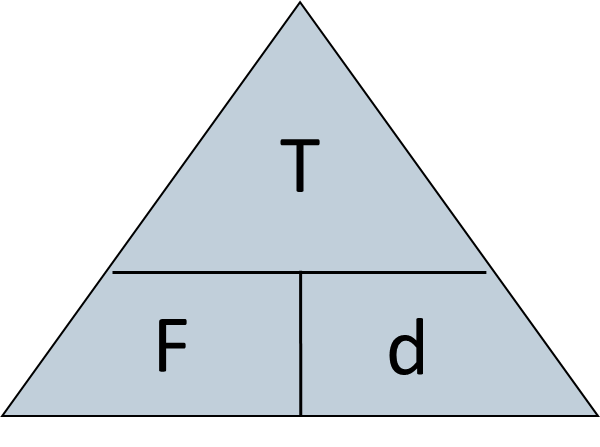
\includegraphics[scale=0.75]{Imagenes/Triangulo_Trabajo.png}
\end{figure}
\pause
\begin{align*}
T = F \cdot d
\end{align*}
\end{frame}
\begin{frame}
\frametitle{Resolviendo el ejercicio}
\textocolor{red}{Sustitución:}
\begin{eqnarray*}
\begin{aligned}
T &= (\SI{5d3}{\newton})(\SI{3d3}{\meter}) = \\[0.5em] \pause 
T &= \SI{15d6}{\newton\meter} = \\[0.5em] \pause 
T &= \SI{15d6}{\joule} 
\end{aligned}
\end{eqnarray*}
\end{frame}
\begin{frame}
\frametitle{Enunciado de otro ejercicio}
Un hombre carga el paquete que recibió a la puerta de su casa, la caja indica el contenido de \SI{55}{\kilo\gram}, recorre \SI{90}{\centi\meter} y lo apoya en la mesa.
\\
\bigskip
\pause
¿Cuánto trabajo realiza el hombre?
\end{frame}
\begin{frame}
\frametitle{Resolviendo el ejercicio}
\textocolor{red}{Datos:}
\pause
\begin{eqnarray*}
\begin{aligned}
m &= \SI{55}{\kilo\gram} \\[0.5em]
d &= \SI{90}{\centi\meter} = \SI{0.9}{\meter} \\[0.5em] \pause
F &= \, ? \\[0.5em]
T &= \, ?
\end{aligned}
\end{eqnarray*}
\end{frame}
\begin{frame}
\frametitle{Resolviendo el ejercicio}
\textocolor{red}{Expresiones:}
\begin{align*}
F &= m \, g \\[0.5em]
T &= F \cdot d
\end{align*}
\end{frame}
\begin{frame}
\frametitle{Resolviendo el ejercicio}
\textocolor{red}{Sustituciones:}
\begin{eqnarray*}
\begin{aligned}
F &= (\SI{55}{\kilo\gram})(\SI[per-mode=fraction]{9.81}{\meter\per\square\second}) = \pause \SI{539.55}{\newton} \\[0.5em] \pause
T &= (\SI{539.55}{\newton})(\SI{0.9}{\meter}) = \pause \SI{485.89}{\joule}
\end{aligned}
\end{eqnarray*}
\end{frame}
% \begin{frame}
% \frametitle{Enunciado de otro ejercicio}
% Para arrancar un auto de \SI{800}{\kilo\gram} de transmisión estándar \enquote{en segunda}, se necesita como mínimo recorrer \SI{5}{\meter} de distancia. \pause Si entre varios amigos realizaron un trabajo de \SI{3.5d4}{\joule} al empujarlo:
% \setbeamercolor{item projected}{bg=electricgreen,fg=black}
% \setbeamertemplate{enumerate items}{%
% \usebeamercolor[bg]{item projected}%
% \raisebox{1.5pt}{\colorbox{bg}{\color{fg}\footnotesize\insertenumlabel}}%
% }
% \begin{enumerate}[<+->]
% \item ¿Lograron que el auto arrancara?
% \item ¿Qué trabajo se requiere exactamente para que el auto arranque?
% \end{enumerate}
% \end{frame}

\section{Energía}
\frame[allowframebreaks]{\tableofcontents[currentsection, hideothersubsections]}
\subsection{Definición}

\begin{frame}
\frametitle{La energía en física}
La \textocolor{cobalt}{energía} es la capacidad para desarrollar un trabajo.
\\
\bigskip
\pause
Su unidad son los Joules (J), que equivalen a un newton por metro (\unit{\newton\meter}).
\end{frame}
\begin{frame}
\frametitle{Energía constante}
La energía que existe en el Universo \textocolor{byzantine}{es constante},\pause es decir, su cantidad total no aumenta ni disminuye.
\end{frame}
\begin{frame}
\frametitle{Ley de conservación de la energía}
La energía existente en el Universo no se crea ni se destruye, sólo se transforma.
\end{frame}

\subsection{Energía cinética}

\begin{frame}
\frametitle{Energía cinética}
Es la energía que genera un cuerpo \textocolor{coolblack}{al estar en movimiento}.
\pause
\begin{align*}
E_{k} = \dfrac{1}{2} m \, v^{2}
\end{align*}
\end{frame}
\begin{frame}
\frametitle{Enunciado del ejercicio}
Calcula la energía cinética de un vehículo de \SI{1000}{\kilo\gram} de masa que circula a una velocidad de \SI{120}{\kilo\meter\per\hour}.
\end{frame}
\begin{frame}
\frametitle{Resolviendo el ejercicio}
\vspace*{-1cm}
\textocolor{red}{Datos:}
\begin{eqnarray*}
\begin{aligned}
m &= \SI{1000}{\kilo\gram} \\ \pause
v &= \SI{120}{\kilo\meter\per\hour} \hspace{1cm} \text{Hay que convertir a } \si{\meter\per\second} \\[0.5em] \pause
v &= \SI[per-mode=fraction]{120}{\kilo\meter\per\hour} \left( \dfrac{\SI{1000}{\meter}}{\SI{1}{\kilo\meter}} \right) (\dfrac{\SI{1}{\hour}}{\SI{3600}{\second}}) = \pause \dfrac{\SI{120000}{\meter}}{\SI{3600}{\second}} = \\ \pause
v &= \SI[per-mode=fraction]{33.33}{\meter\per\second}
\end{aligned}
\end{eqnarray*}
\end{frame}
\begin{frame}
\frametitle{Resolviendo el ejercicio}
\textocolor{red}{Expresión:}
\begin{align*}
E_{k} = \dfrac{1}{2} m \, v^{2}
\end{align*}
\end{frame}
\begin{frame}
\frametitle{Resolviendo el ejercicio}
\vspace*{-1cm}
\textocolor{red}{Sustitución:}
\pause
\begin{eqnarray*}
\begin{aligned}
E_{k} &= \dfrac{1}{2} (\SI{1000}{\kilo\gram}) \left( \SI[per-mode=fraction]{33.33}{\meter\per\second} \right)^{2} = \\[0.5em] \pause
E_{k} &= \dfrac{1}{2} (\SI{1000}{\kilo\gram}) \left( \SI[per-mode=fraction]{1110.88}{\square\meter\per\square\second} \right) = \\[0.5em] \pause
E_{k} &= \dfrac{1}{2} \left( \SI[per-mode=fraction]{1110888.9}{\kilo\gram\square\meter\per\square\second} \right) = \\[0.5em] \pause
E_{k} &= \SI{555444.45}{\joule}
\end{aligned}
\end{eqnarray*}
\end{frame}
\begin{frame}
\frametitle{Enunciado de otro ejercicio}
Calcula la velocidad a la que va trotando una persona de \SI{65}{\kilo\gram} para que adquiera una energía cinética de \SI{700}{\joule}.
\end{frame}
\begin{frame}
\frametitle{Resolviendo el ejercicio}
\vspace*{-1cm}
\textocolor{red}{Datos:} \pause m = \SI{65}{\kilo\gram}, \pause $E_{k} = \SI{700}{\joule}$
\\
\bigskip
\pause
\textocolor{red}{Expresión:}
\begin{eqnarray*}
\begin{aligned}
E_{k} &= \dfrac{1}{2} m \, v^{2} \pause \hspace{1cm} \Rightarrow \hspace{0.5cm} \, v^{2} = 2 \, E_{k} \\[0.5em] \pause
\Rightarrow v^{2} &= \dfrac{2 \, E_{k}}{m} \\[0.5em] \pause
v &= \sqrt{\dfrac{2 \, E_{k}}{m}}
\end{aligned}
\end{eqnarray*}
\end{frame}
\begin{frame}
\frametitle{Resolviendo el ejercicio}
\textocolor{red}{Sustitución:}
\pause
\begin{eqnarray*}
\begin{aligned}
v &= \sqrt{\dfrac{2 \, \SI{700}{\joule}}{\SI{65}{\kilo\gram}}} = \pause \sqrt{\dfrac{2 \, \SI{700}{\newton\meter}}{\SI{65}{\kilo\gram}}} = \\[0.5em]\pause 
v &= \sqrt{\dfrac{\displaystyle 2 \, \SI[per-mode=fraction]{700}{\kilo\gram\square\meter\per\square\second}}{\SI{65}{\kilo\gram}}} = \pause \sqrt{\num{21.53} \, \dfrac{\text{kg m}^{2}}{\text{kg s}^{2}}} = \\[0.5em] \pause
v &= \SI[per-mode=fraction]{4.64}{\meter\per\second}
\end{aligned}
\end{eqnarray*}
\end{frame}    

\subsection{Energía potencial}

\begin{frame}
\frametitle{Definición de la energía potencial}
Es la energía que tiene un cuerpo por su posición, \textocolor{cadmiumgreen}{con respecto de la horizontal o altura}, es también llamada energía gravitatoria.
\end{frame}
\begin{frame}
\frametitle{Expresión para la energía potencial}
Para obtener la energía potencial $E_{p}$, se ocupa la siguiente expresión:
\pause
\begin{align*}
E_{p} = m \, g \, h
\end{align*}
\end{frame}
\begin{frame}
\frametitle{Enunciado del ejercicio}
Calcula la energía potencial que posee un libro de \SI{500}{\gram} de masa que está colocado sobre una mesa de \SI{80}{\centi\meter} de altura.
\end{frame}
\begin{frame}
\frametitle{Resolviendo el ejercicio}
\textocolor{red}{Datos:} \pause m = \SI{50}{\gram}, \pause \hspace{0.5cm} $h = \SI{80}{\centi\meter}$, \pause \hspace{0.5cm} $g = \SI{9.81}{\meter\per\square\second}$
\\
\bigskip
\pause
\textocolor{red}{Expresión:}
\begin{eqnarray*}
\begin{aligned}
E_{p} &= m \, g \, h
\end{aligned}
\end{eqnarray*}
\end{frame}
\begin{frame}
\frametitle{Resolviendo el ejercicio}
\textocolor{red}{Sustitución:}
\pause
\begin{eqnarray*}
\begin{aligned}
E_{p} &= (\SI{0.5}{\kilo\gram}) \left( \SI[per-mode=fraction]{9.81}{\meter\per\square\second} \right) (\SI{0.8}{\meter}) = \\[0.5em] \pause
E_{p} &= \SI{3.92}{\joule}
\end{aligned}
\end{eqnarray*}
\end{frame}
% \begin{frame}
% \frametitle{Ejercicio por resolver}
% ¿En qué piso de un estacionamiento se encuentra un auto de \SI{840}{\kilo\gram} para que se energía potencial sea de \SI{39600}{\joule}?
% \\
% \bigskip
% Cada piso mide \SI{2.4}{\meter}
% \end{frame}
% \begin{frame}
% \frametitle{Ejercicio por resolver}
% Calcula la masa de un objeto que se levanta hasta una altura de \SI{12}{\meter} que adquiere una energía potencial de \SI{2120}{\joule}.
% \end{frame}
% \begin{frame}
% \frametitle{Ejercicio por resolver}
% Un balón de \SI{600}{\gram} se patea hacia arriba con una velocidad de \SI{35}{\meter\per\second}. \pause Calcula:
% \pause
% \setbeamercolor{item projected}{bg=bananayellow,fg=black}
% \setbeamertemplate{enumerate items}{%
% \usebeamercolor[bg]{item projected}%
% \raisebox{1.5pt}{\colorbox{bg}{\color{fg}\footnotesize\insertenumlabel}}%
% }
% \begin{enumerate}[<+->]
% \item El valor inicial de las energías cinética y potencial.
% \seti
% \end{enumerate}
% \end{frame}
% \begin{frame}
% \frametitle{Ejercicio por resolver}
% \setbeamercolor{item projected}{bg=bananayellow,fg=black}
% \setbeamertemplate{enumerate items}{%
% \usebeamercolor[bg]{item projected}%
% \raisebox{1.5pt}{\colorbox{bg}{\color{fg}\footnotesize\insertenumlabel}}%
% }
% \begin{enumerate}[<+->]    
% \conti
% \item La energía cinética y potencial a los \SI{20}{\meter} de altura.
% \item Demuestra que la energía mecánica se conserva.
% \end{enumerate}
% \end{frame}

\section{Temperatura}
\frame[allowframebreaks]{\tableofcontents[currentsection, hideothersubsections]}
\subsection{La temperatura}

\begin{frame}
\frametitle{Definición de temperatura}
La \textocolor{darkgreen}{temperatura} es una magnitud física que nos indica qué tan caliente o frío se encuentra un cuerpo o una sustancia.
\end{frame}

\subsection{Escalas de temperatura}

\begin{frame}
\frametitle{Las escalas de temperatura}
Para medir la temperatura hay diferentes escalas, la más usuales son:
\end{frame}
\begin{frame}
\frametitle{Las escalas de temperatura}
\setbeamercolor{item projected}{bg=lilac,fg=black}
\setbeamertemplate{enumerate items}{%
\usebeamercolor[bg]{item projected}%
\raisebox{1.5pt}{\colorbox{bg}{\color{fg}\footnotesize\insertenumlabel}}%
}
\begin{enumerate}[<+->]
\item Celsius.
\item Fahrenheit.
\item Kelvin.
\item Rankine.
\end{enumerate}
\end{frame}

\subsection{Escala Celsius}

\begin{frame}
\frametitle{La escala Celsius}
Para medir la temperatura hay diferentes escalas, la más usual es la \textocolor{brown(web)}{escala Celsius}, \pause que marca \SI{0}{\degreeCelsius} cuando el agua se congela \pause y \SI{100}{\degreeCelsius} cuando ésta hierve.
\end{frame}
\begin{frame}
\frametitle{La escala Celsius}
La distancia entre los dos límites se divide en cien partes iguales. 
\\
\bigskip
\pause
Cada una corresponde a un grado centígrado.
\end{frame}

\subsection{Escala Fahrenheit}

\begin{frame}
\frametitle{La escala Fahrenheit}
En Estados Unidos y en Europa se utiliza la \textocolor{burgundy}{escala Fahrenheit}.%; \pause fue establecida por el físico holandés-alemán Gabriel Daniel Fahrenheit en 1724.
\end{frame}
\begin{frame}
\frametitle{Conversión entre escalas}
Para convertir temperaturas entre las escalas Celsius y Fahrenheit, se utilizan las siguientes expresiones:
\pause
\begin{eqnarray*}
\begin{aligned}
\unit{\degreeCelsius} &= \dfrac{5}{9} \left( ^{\circ}\text{F} - 32 \right) \\[0.5em] \pause
^{\circ}\text{F} &= \dfrac{9}{5} \, \unit{\degreeCelsius} + 32
\end{aligned}
\end{eqnarray*}
\end{frame}
\begin{frame}
\frametitle{Ejercicio 1}
Si la temperatura interior de una casa es de \SI{10}{\degreeCelsius}.
\\
\bigskip
\pause
¿Cuál será la temperatura en escala Fahrenheit?
\end{frame}
\begin{frame}
\frametitle{Solución al ejercicio}
Datos del enunciado: $T = \SI{10}{\degreeCelsius}$
\\
\bigskip
\pause
Expresión:
\pause
\begin{align*}
^{\circ}\text{F} &= \dfrac{9}{5} \, \unit{\degreeCelsius} + 32
\end{align*}
\end{frame}
\begin{frame}
\frametitle{Solución al ejercicio}
Sustitución:
\pause
\begin{eqnarray*}
\begin{aligned}
^{\circ}\text{F} &= \left( \dfrac{9}{5}\right) \left( \SI{10}{\degreeCelsius} \right) + 32 = \\[0.5em] \pause
&= 18 + 32 = \\[0.5em] \pause
&=50 ^{\circ} \text{F}
\end{aligned}
\end{eqnarray*}
\end{frame}
\begin{frame}
\frametitle{Ejercicio 2}
La temperatura en verano en la ciudad de Puerto Vallarta ha llegado a alcanzar los $110 ^{\circ} \text{F}$.
\\
\bigskip
\pause
Expresa esta temperatura en grados Celsius.
\end{frame}
\begin{frame}
\frametitle{Resolviendo el Ejercicio}
Datos: $T = 110 ^{\circ} \text{F}$
\\
\bigskip
\pause
Expresión:
\pause
\begin{align*}
\unit{\degreeCelsius} &= \dfrac{5}{9} \left( ^{\circ}\text{F} - 32 \right)
\end{align*}
\end{frame}
\begin{frame}
\frametitle{Resolviendo el Ejercicio}
Sustitución:
\pause
\begin{eqnarray*}
\begin{aligned}
\unit{\degreeCelsius} &= \left( \dfrac{5}{9} \right) \left( 110 - 32 \right) = \\[0.5em] \pause
&= \left( \dfrac{5}{9} \right) \left( 78 \right) = \\[0.5em] \pause
&= \SI{43.33}{\degreeCelsius}
\end{aligned}
\end{eqnarray*}
\end{frame}

\subsection{Escala Kelvin}

\begin{frame}
\frametitle{Definiendo la escala Kelvin}
Las unidades en la escala Kelvin son de la misma equivalencia que las unidades de la escala Celsius y se simbolizan con la letra K.
\end{frame}
\begin{frame}
\frametitle{Definiendo la escala Kelvin}    
La temperatura de fusión del hielo es de \SI{273.15}{\kelvin}, \pause de tal forma que cero grados Kelvin corresponden a \SI{-273.15}{\degreeCelsius}. 
\end{frame}
\begin{frame}
\frametitle{Relación entre escalas}
La relación entre la escala Celsius y la escala Kelvin es:
\pause
\begin{eqnarray*}
\begin{aligned}
K &= \unit{\degreeCelsius} + 273.15 \\[0.5em]
\unit{\degreeCelsius} &= K - 273.15
\end{aligned}
\end{eqnarray*}
\end{frame}
\begin{frame}
\frametitle{Ejercicio a cuenta}
Resuelve las siguientes conversiones de temperatura, indicando todo el procedimiento necesario:
\pause
\begin{multicols}{2}
\setbeamercolor{item projected}{bg=blue,fg=white}
\setbeamertemplate{enumerate items}{%
\usebeamercolor[bg]{item projected}%
\raisebox{1.5pt}{\colorbox{bg}{\color{fg}\footnotesize\insertenumlabel}}%
}
\begin{enumerate}
\item \SI{50}{\degreeCelsius} a \unit{\kelvin}
\item \SI{120}{\degreeCelsius} a \unit{\kelvin}
\item \SI{380}{\kelvin} a \unit{\degreeCelsius}
\item \SI{210}{\kelvin} a \unit{\degreeCelsius}
\item \SI{60}{\degreeCelsius} a $^{\circ}$F
\item \SI{98}{\degreeCelsius} a $^{\circ}$F
\item $50^{\circ}$ F a \unit{\degreeCelsius}
\item $130^{\circ}$ F a \unit{\degreeCelsius}    
\end{enumerate}
\end{multicols}
\end{frame}

\subsection{Escala Rankine}

\begin{frame}
\frametitle{Definiendo la escala Rankine}
La \textocolor{byzantium}{escala Rankine} se define midiendo en grados Fahrenheit sobre el cero absoluto.
\end{frame}
\begin{frame}
\frametitle{Definiendo la escala Rankine}
En esta escala tampoco se introducen valores negativos de temperatura, \pause por lo que ambas se consideran escalas de temperatura absoluta.
\end{frame}
\begin{frame}
\frametitle{Relación entre escalas}
La relación entre la escala Rankine y la escala Fahrenheit es:
\pause
\begin{align*}
R = \, ^{\circ}\text{F} + 460
\end{align*}
\end{frame}
\begin{frame}
\frametitle{Ejercicio}
La temperatura de ebullición del agua es de $212 ^{\circ}\text{F}$,
\\
\bigskip
\pause
¿Cuál será la temperatura en escala Rankine?
\end{frame}
\begin{frame}
\frametitle{Resolviendo el ejercicio}
\textocolor{red}{Datos:} $T = 212 ^{\circ}\text{F}$  \\[0.5em]\pause
\textocolor{red}{Expresión:} $R = \, ^{\circ}\text{F} + 460$ \\[0.5em]\pause
\textocolor{red}{Sustitución:} $R = 212 + 460 = 672 \, R$
\end{frame}
% \begin{frame}
% \frametitle{Ejercicio a cuenta}
% Completa la siguiente tabla, escribiendo en cada celda el valor de temperatura correspondiente.
% \\
% \bigskip
% \pause
% Deberás de incluir las operaciones necesarias.
% \end{frame}
% \begin{frame}
% \frametitle{Ejercicio a cuenta}
% \begin{table}
% \fontsize{10}{10}\selectfont
% \centering
% \begin{tabular}{| l | c | c | c | c |} \hline
% Temperatura & \unit{\degreeCelsius} & $^{\circ}$ F & K & R \\ \hline
% Ebullición del oro & & & $3129$ & \\ \hline
% Ebullición del n-butanol & $117.4$ & & & \\ \hline
% Temperatura corporal del cuerpo humano & & $98.6$ & & \\ \hline
% Ebullición del agua en la ciudad de Puebla & & & $366$ & \\ \hline
% Temperatura ambiente en la ciudad de Puebla & & & & $18$ \\ \hline
% \end{tabular}
% \end{table}
% \end{frame}

\section{El calor}
\frame{\tableofcontents[currentsection, hideothersubsections]}
\subsection{Definición}

\begin{frame}
\frametitle{Definición de calor}
El \textocolor{burntorange}{calor} es la transferencia de energía de un cuerpo a otro debido a que hay una
diferencia de temperatura entre ambos.
\end{frame}
\begin{frame}
\frametitle{Unidades de calor}
Las unidades de calor son:
\pause
\begin{eqnarray*}
\begin{aligned}
\text{MKS} \quad &\Rightarrow \text{Joule} \, \quad \unit{\joule}  \quad \left[ \SI{1}{\newton\metre} \right] \\[0.5em] \pause
\text{cgs} \quad &\Rightarrow \text{ergio} \, \quad \unit{\erg} \quad \left[ 1 \, \text{din} \, \unit{\centi\metre} \right]
\end{aligned}
\end{eqnarray*}
\end{frame}

\subsection{Tipos de transferencia}


\begin{frame}
\frametitle{Tipos de transferencia}
El calor se transfiere entre los cuerpos en tres tipos distintos de procesos:
\pause
\setbeamercolor{item projected}{bg=carmine,fg=white}
\setbeamertemplate{enumerate items}{%
\usebeamercolor[bg]{item projected}%
\raisebox{1.5pt}{\colorbox{bg}{\color{fg}\footnotesize\insertenumlabel}}%
}
\begin{enumerate}[<+->]
\item Conducción.
\item Radiación.
\item Convección.
\end{enumerate}
\end{frame}
\begin{frame}
\frametitle{Conducción de calor}
Es el proceso mediante el cual el calor \textocolor{cadmiumgreen}{se transfiere directamente} a través de un material, \pause sin ningún
movimiento neto del material.
\end{frame}
% \begin{frame}
% \frametitle{Conducción de calor}    
% Por ejemplo, si acercas una varilla de metal a una flama, el calor que la flama emite se conduce al metal y éste a tu mano.
% \end{frame}
\begin{frame}
\frametitle{Conducción de calor}
\begin{figure}
    \centering
    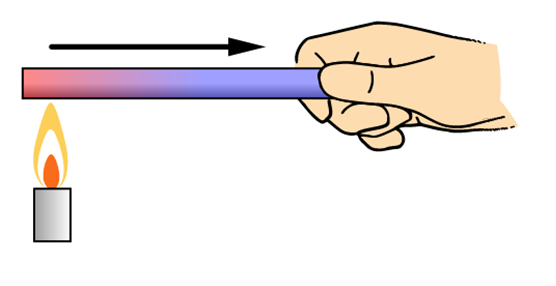
\includegraphics[scale=0.5]{Imagenes/Calor_03.png}
\end{figure}
\end{frame}
\begin{frame}
\frametitle{Radiación de calor}
Es el proceso por el que los cuerpos \textocolor{cadmiumred}{emiten energía} que puede propagarse por el vacío.
\\
\bigskip
\pause
La energía radiante se transporta mediante ondas electromagnéticas.
\end{frame}
% \begin{frame}
% \frametitle{Radiación de calor}
% Por ejemplo, por la radiación nos llega el calor del sol, \pause así como también por la radiación podemos sentir el calor que se desprende de un foco encendido si acercamos la mano.
% \end{frame}
\begin{frame}
\frametitle{Radiación de calor}
\begin{figure}
    \centering
    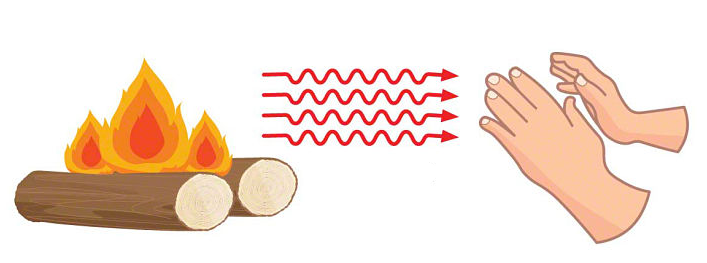
\includegraphics[scale=0.5]{Imagenes/Calor_02.png}
\end{figure}
\end{frame}
\begin{frame}
\frametitle{Convección de calor}
Es el proceso por el cual el calor \textocolor{carmine}{se transfiere a través de un fluido} por el movimiento del mismo.
\end{frame}
% \begin{frame}
% \frametitle{Convección de calor}
% Por ejemplo, cuando se pone a calentar un recipiente con agua, \pause ésta al calentarse en la parte inferior se dilata y disminuye su densidad.
% \end{frame}
\begin{frame}
\frametitle{Convección de calor}
\begin{figure}
    \centering
    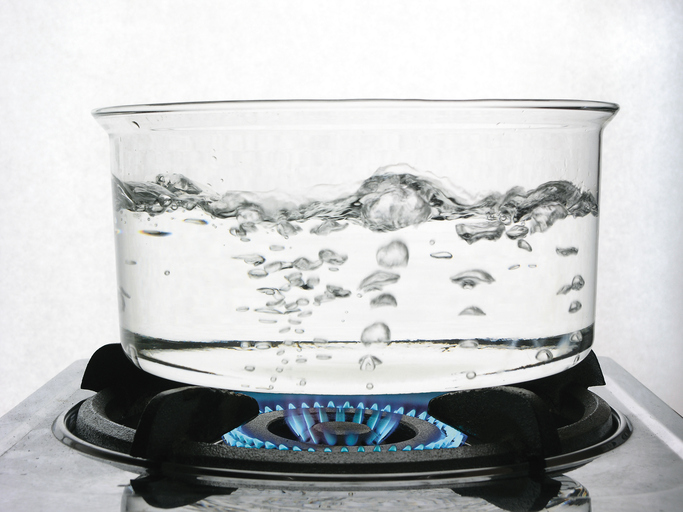
\includegraphics[scale=0.25]{Imagenes/Calor_01.jpg}
\end{figure}
\end{frame}
\begin{frame}
\frametitle{Convección de calor}
Por lo que el agua caliente asciende y transporta así el calor de la parte inferior a la parte superior, \pause generando un movimiento interno de las partículas.
\end{frame}

\end{document}